\documentclass[dvisvgm,tikz]{standalone}
\begin{document}
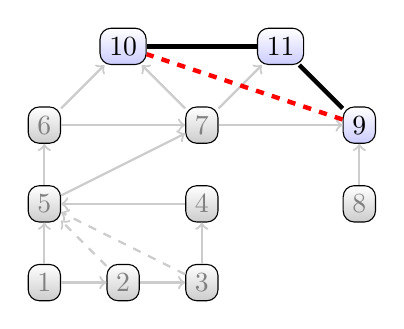
\begin{tikzpicture}

\node[shape=rectangle, rounded corners, draw, align=center, top color=white, bottom color=black!20, text=black!50] (n1) at (0.0,0.0) {1};
\node[shape=rectangle, rounded corners, draw, align=center, top color=white, bottom color=black!20, text=black!50] (n2) at (1.0,0.0) {2};
\node[shape=rectangle, rounded corners, draw, align=center, top color=white, bottom color=black!20, text=black!50] (n3) at (2.0,0.0) {3};
\node[shape=rectangle, rounded corners, draw, align=center, top color=white, bottom color=black!20, text=black!50] (n4) at (2.0,1.0) {4};
\node[shape=rectangle, rounded corners, draw, align=center, top color=white, bottom color=black!20, text=black!50] (n5) at (0.0,1.0) {5};
\node[shape=rectangle, rounded corners, draw, align=center, top color=white, bottom color=black!20, text=black!50] (n6) at (0.0,2.0) {6};
\node[shape=rectangle, rounded corners, draw, align=center, top color=white, bottom color=black!20, text=black!50] (n7) at (2.0,2.0) {7};
\node[shape=rectangle, rounded corners, draw, align=center, top color=white, bottom color=black!20, text=black!50] (n8) at (4.0,1.0) {8};
\node[shape=rectangle, rounded corners, draw, align=center, top color=white, bottom color=blue!20] (n9) at (4.0,2.0) {9};
\node[shape=rectangle, rounded corners, draw, align=center, top color=white, bottom color=blue!20] (n10) at (1.0,3.0) {10};
\node[shape=rectangle, rounded corners, draw, align=center, top color=white, bottom color=blue!20] (n11) at (3.0,3.0) {11};
\draw[thick,black!20,->] (n1) -- (n2);
\draw[thick,black!20,->] (n1) -- (n5);
\draw[thick,black!20,->] (n2) -- (n3);
\draw[thick,black!20,dashed,->] (n2) -- (n5);
\draw[thick,black!20,->] (n3) -- (n4);
\draw[thick,black!20,dashed,->] (n3) -- (n5);
\draw[thick,black!20,->] (n4) -- (n5);
\draw[thick,black!20,->] (n5) -- (n6);
\draw[thick,black!20,->] (n5) -- (n7);
\draw[thick,black!20,->] (n6) -- (n7);
\draw[thick,black!20,->] (n6) -- (n10);
\draw[thick,black!20,->] (n7) -- (n9);
\draw[thick,black!20,->] (n7) -- (n10);
\draw[thick,black!20,->] (n7) -- (n11);
\draw[thick,black!20,->] (n8) -- (n9);
\draw[ultra thick,red,dashed] (n9) -- (n10);
\draw[ultra thick] (n9) -- (n11);
\draw[ultra thick] (n10) -- (n11);
\end{tikzpicture}
\end{document}

